\documentclass[letterpaper, 11pt]{article}
\usepackage[utf8]{inputenc}
\usepackage[letterpaper, portrait, margin=1in]{geometry}
\usepackage{pgfplots}
\pgfplotsset{width=10cm,compat=1.9}
\usepackage{hyperref}
\usepackage{textcomp}
\usepackage{siunitx}
\usepackage{amsmath}
\usepackage{cancel}
\usepackage{tikz}
\usepackage{everysel}
\usepackage{ragged2e}
\usepackage{mathdots}
\usepackage{yhmath}
\usepackage{color}
\usepackage{array}
\usepackage{multirow}
\usepackage{amssymb}
\usepackage{gensymb}
\usepackage{tabularx}
\usepackage{booktabs}
\usepackage{listings}
\usepackage{xcolor}
\usepackage{enumitem}
\usetikzlibrary{fadings}
\usetikzlibrary{patterns}
\usetikzlibrary{shadows.blur}
\hypersetup{
    colorlinks=true,
    linkcolor=black,
    filecolor=black,      
    urlcolor=blue,
}

\definecolor{codegreen}{rgb}{0,0.6,0}
\definecolor{codegray}{rgb}{0.5,0.5,0.5}
\definecolor{codepurple}{rgb}{0.58,0,0.82}
\definecolor{backcolour}{rgb}{0.95,0.95,0.92}

\lstdefinestyle{mystyle}{
    backgroundcolor=\color{backcolour},   
    commentstyle=\color{codegreen},
    keywordstyle=\color{magenta},
    numberstyle=\tiny\color{codegray},
    stringstyle=\color{codepurple},
    basicstyle=\ttfamily\footnotesize,
    breakatwhitespace=false,         
    breaklines=true,                 
    captionpos=b,                    
    keepspaces=true,                 
    numbers=left,                    
    numbersep=5pt,                  
    showspaces=false,                
    showstringspaces=false,
    showtabs=false,                  
    tabsize=2
}

\lstset{style=mystyle}

\title{COMSC-200 \\ Lab 9}
\author{Ryan Jacoby}
\date{8 November 2020}
\begin{document}

\maketitle

\section{Shifting and Printing an Integer}
Write a program that right-shifts an integer variable four bits.  The program should print the integer before and after the shift operation.  Does your system place zeros or ones in the vacated bits. \\

My system places 0s in the vacated bits; 255(b11111111) becomes 15(b00001111).

\begin{lstlisting}[language=c++, caption=main.cpp]
// Ryan Jacoby

#include<iostream>

using namespace std;

int main() {
    int val;
    cout << "Enter a value to be bitshifted: ";
    cin >> val;
    
    val = val >> 4;
    cout << "Your value bitshifted 4 itmes is: " << val << '\n';
    return 0;
}
\end{lstlisting}

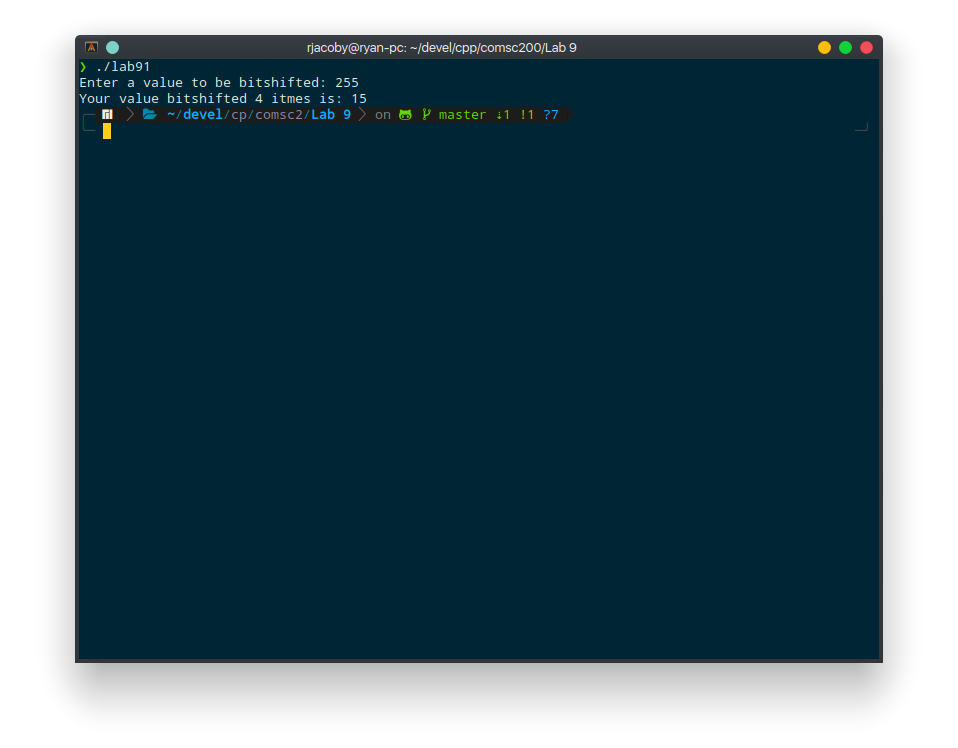
\includegraphics[scale=0.5]{right_shift.png}

\section{Multiplication Via Bit Shifting}
Left-shifting an unsigned integer by one bit is equivalent to multiplying the value by 2.  Write a function power2 that takes two integer arguments, \textit{number} and \textit{pow} and calculates $number * 2^{pow}$.  Use a shift operator to calculate the result.  The program should print the values as integers and as bits.

\begin{lstlisting}[language=c++, caption=main.cpp]
// Ryan Jacoby

#include<iostream>

using namespace std;

int power2(int, int);
void print_16bit(int);

int main() {
    int a, b;
    cout << "Enter an integer: ";
    cin >> a;

    cout << "Enter another integer: ";
    cin >> b;

    cout << "A: " << a << "\tb";
    print_16bit(a);

    cout << "\nB: " << b << "\tb";
    print_16bit(b);

    cout << "\n\n A * 2^B = " << power2(a, b) << "\tb";
    print_16bit(power2(a, b));
    cout << '\n';
    return 0;
}

int power2(int number, int pow) {
    return number << pow;
}

void print_16bit(int n) {
    for(int i = 15; i >= 0; i--) cout << ((n >> i) & 1U);
}
\end{lstlisting}

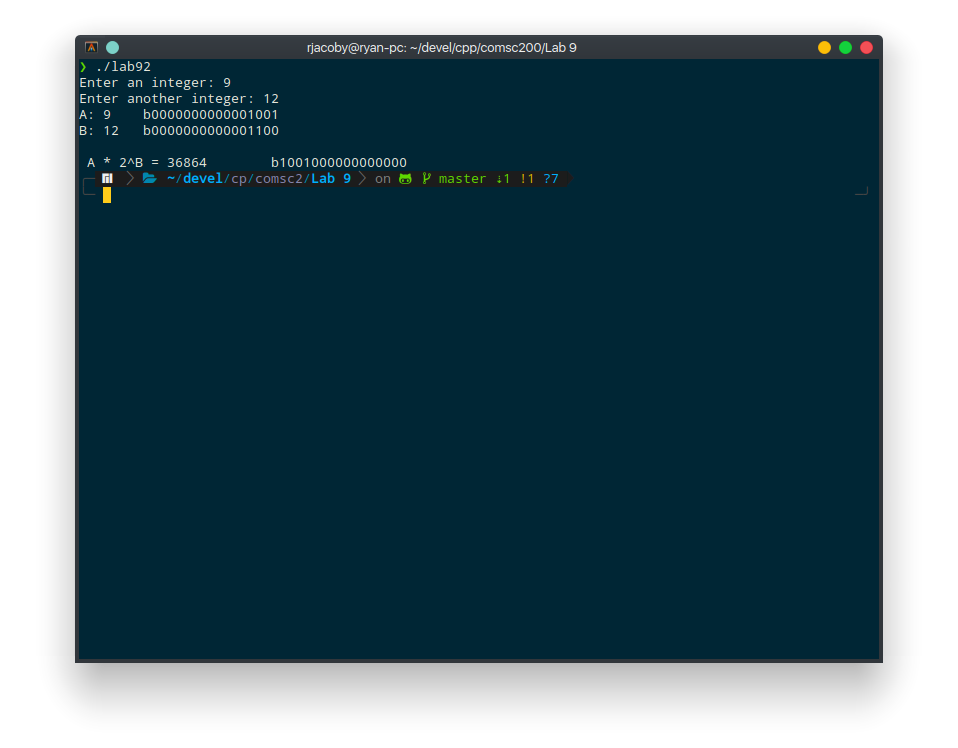
\includegraphics[scale=0.5]{pow.png}

\section{Even Parity Simulation}

\begin{lstlisting}[language=c++, caption=main.cpp]
// Ryan Jacoby

#include<iostream>
#include<ctime>

using namespace std;

int power2(int, int);
void print_32bit(int);
int count1(int);
unsigned int parity_enc(unsigned int *);
bool parity_dec(unsigned int);
int randomize(int);


int main() {
    srand(time(NULL));
    
    int correct = 0;

    for(int i = 0; i < 10000; i++) {
        unsigned int n = rand() % (1 << 30);
        parity_enc(&n);
        n = randomize(n);

        if(parity_dec(n)) correct++;
    }

    cout << "Percent transmission: " << correct / 100.0 << "%\n";

    return 0;
}

int power2(int number, int pow) {
    return number << pow;
}

void print_32bit(int n) {
    for(int i = 31; i >= 0; i--) cout << ((n >> i) & 1U);
}

int count1(int n) {
    int ret = 0;
    for(int i = 31; i >= 0; i--) if((n >> i) & 1U == 1) ret++;
    return ret;
}

unsigned int parity_enc(unsigned int * n) {
    if(count1(*n) % 2 == 1) { 
        *n = (*n | (1 << 31));
        return *n;
    }
    return *n;
}

bool parity_dec(unsigned int n) { 
    return count1(n) % 2 == 0;
}

int randomize(int n) {
    if(rand() % 10 == 0) return (1 << rand() % 32) ^ n;
    return n;
}
\end{lstlisting}

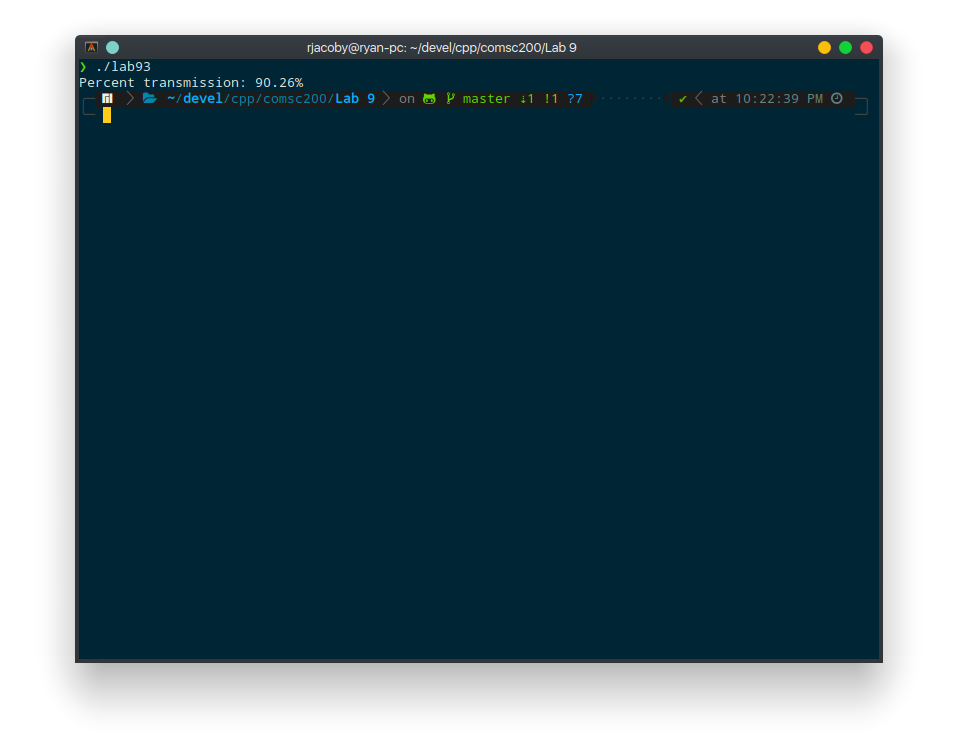
\includegraphics[scale=0.5]{parity.png}

\end{document}
